\documentclass[12pt,addpoints]{evalua}
\grado{3$^\circ$ de Primaria}
\cicloescolar{2024-2025}
\materia{Matemáticas}
\unidad{}
\title{Examen General}
\aprendizajes{\footnotesize%
   \item Expresa oralmente la sucesión numérica hasta cuatro cifras, en español y hasta donde sea posible, en su lengua materna, de manera ascendente y descendente a partir de un número natural dado.\\[-1.8em]
   \item Representa, con apoyo de material concreto y modelos gráficos, fracciones: medios, cuartos, octavos, dieciseisavos, para expresar el resultado de mediciones y repartos en situaciones vinculadas a su contexto.\\[-1.8em]
   \item Resuelve situaciones problemáticas vinculadas a su contexto que implican sumas, restas, multiplicación y división de números naturales de hasta tres cifras utilizando el algoritmo convencional y que impliquen, medición, estimación y comparación, de longitudes, masas y capacidades, con el uso del metro, kilogramo, litro y medios y cuartos de estas unidades; en el caso de la longitud, el decímetro y centímetro.\\[-1.8em]
   \item Resuelve problemas de suma, resta, multiplicación y división vinculados a su contexto, que impliquen el uso de fracciones (medios, cuartos, octavos, dieciseisavos), con el apoyo de material concreto o representaciones gráficas.
      }
\author{Prof.: Julio César Melchor Pinto}
\begin{document}%
\vfill
\tableofcontents
\afterpage{\blankpage}
\begin{questions}\large
	\addcontentsline{toc}{section}{Unidad 1}
	\section*{Unidad 1}
	\addcontentsline{toc}{subsection}{Escritura de cantidades}
	\subsection*{Escritura de cantidades}

	\question[6]{Escribe sore la línea los siguientes números

		\begin{multicols}{2}
			\begin{parts}%\large
				\part \fillin[  65][1.5cm] Sesenta y cinco.
				\part \fillin[ 109][1.5cm] Ciento nueve.
				\part \fillin[ 254][1.5cm] Doscientos cincuenta y cuatro.
				\part \fillin[ 314][1.5cm] Trescientos catorce.
				\part \fillin[ 431][1.5cm] Cuatrocientos treinta y uno.
				\part \fillin[1024][1.5cm] Mil veinticuatro.
			\end{parts}
		\end{multicols}
	}

	\addcontentsline{toc}{subsection}{Sistema decimal}
	\subsection*{Sistema decimal}

	\question[4]{Señala la opción que responda correctamente a cada una de las siguientes preguntas:

		\begin{multicols}{2}
			\begin{parts}%\large
				\part ¿Qué lugar ocupa el 6 en 64?       \fillin[B][0.5cm]
				\part ¿Qué lugar ocupa el 2 en 206?      \fillin[C][0.5cm]
				\part ¿Qué lugar ocupa el 5 en 5138?     \fillin[D][0.5cm]
				% \part ¿Qué lugar ocupa el 2 en 87264?    \fillin[D][0.5cm]
				\part ¿Qué lugar ocupa el 1 en 2331?     \fillin[A][0.5cm]
				% \part ¿Qué lugar ocupa el 8 en 198114?   \fillin[C][0.5cm]
				% \part ¿Qué lugar ocupa el 7 en 46878?    \fillin[E][0.5cm]
				% \part ¿Qué lugar ocupa el 4 en 149778?   \fillin[B][0.5cm]
			\end{parts}

			\columnbreak%

			\begin{choices}%\large
				\choice {\color{Goldenrod}Unidades.}
				\choice {\color{blue}Decenas.}
				\choice {\color{red}Centenas.}
				\choice {\color{Goldenrod}Unidades de millar.}
				% \choice {\color{blue}decenas de millar.}	
				% \choice {\color{red}centenas de millar.}
			\end{choices}
		\end{multicols}
	}

	% \newpage

	\question[6]{Escribe la notación desarrollada de cada uno de los siguientes números:

		\begin{multicols}{2}
			\begin{parts}%\large
				\part $84=$ \fillin[$80+4$][2.4in]\\[0.5em]
				\part $936 =$ \fillin[$900+30+6$][2.4in]\\[0.5em]
				\part $2096=$ \fillin[$2000+90+6$][2.4in]\\[0.5em]
				\part $6215 =$ \fillin[$6000+200+10+5$][2.4in]\\[0.5em]
				\part $4818 =$ \fillin[$4000+800+10+8$][2.4in]\\[0.5em]
				\part $7145 =$ \fillin[$7000+100+40+5$][2.4in]\\[0.5em]
				% \part $5454 =$ \fillin[$5000+400+50+4$][2.4in]
				% \part $6451 =$ \fillin[$6000+400+50+1$][2.4in]
				% \part $19679=$ \fillin[$10000+9000+600+70+9$][2.4in]
				% \part $26324=$ \fillin[$20000+6000+300+20+4$][2.4in]
				% \part $5717 =$ \fillin[$5000+700+10+7$][2.4in]
				% \part $31126=$ \fillin[$30000+1000+100+20+6$][2.4in]
			\end{parts}
		\end{multicols}
	}

	\question[6]{Señala la opción que responda correctamente a cada una de las siguientes preguntas:

		\begin{multicols}{2}
			\begin{parts}%\large
				\part En el número 9658, ¿qué número ocupa la posición de las decenas?

				\begin{oneparcheckboxes}
					\CorrectChoice 5 \choice 6 \choice 8 \choice 9
				\end{oneparcheckboxes}

				\part En el número 7841, ¿qué número ocupa la posición de las unidades de millar?

				\begin{oneparcheckboxes}
					\choice 1 \choice 4  \CorrectChoice 7 \choice 8
				\end{oneparcheckboxes}

				\part En el número 1984, ¿qué número ocupa la posición de las centenas?

				\begin{oneparcheckboxes}
					\choice 1 \choice 4 \choice 8 \CorrectChoice 9
				\end{oneparcheckboxes}

				\part En el número 8147, ¿qué número ocupa la posición de las decenas?

				\begin{oneparcheckboxes}
					\choice 1 \CorrectChoice 4 \choice 7 \choice 8
				\end{oneparcheckboxes}

				\part En el número 2198, ¿qué número ocupa la posición de las centenas?

				\begin{oneparcheckboxes}
					\choice 1 \choice 2  \choice 8 \CorrectChoice 9
				\end{oneparcheckboxes}

				\part En el número 3612, ¿qué número ocupa la posición de las unidades?

				\begin{oneparcheckboxes}
					\choice 1 \CorrectChoice 2 \choice 3 \choice 6
				\end{oneparcheckboxes}

			\end{parts}
		\end{multicols}
	}



	% \subsection*{Sistema decimal 2}
	% \subsubsection*{Posicionamiento decimal 1 }
	% \subsubsection*{Posicionamiento decimal 2 }

	% \question[3]{Señala la opción que responda correctamente a cada una de las siguientes preguntas:

	% 	\begin{multicols}{2}
	% 		\begin{parts}\large
	% 			\part En el número 1.829, ¿qué número ocupa la posición de las centésimas?

	% 			\begin{oneparcheckboxes}
	% 				\choice 1 \CorrectChoice 2 \choice 6 \choice 8 \choice 9
	% 			\end{oneparcheckboxes}

	% 			\part En el número 2.087, ¿qué número ocupa la posición de las décimas?

	% 			\begin{oneparcheckboxes}
	% 				\CorrectChoice 0 \choice 2 \choice 7 \choice 8 \choice 9
	% 			\end{oneparcheckboxes}

	% 			\part En el número 5.928, ¿qué número ocupa la posición de las décimas?

	% 			\begin{oneparcheckboxes}
	% 				\choice 5 \choice 2 \choice 6 \choice 8 \CorrectChoice 9
	% 			\end{oneparcheckboxes}

	% 			\part En el número 3.284, ¿qué número ocupa la posición de las milésimas?

	% 			\begin{oneparcheckboxes}
	% 				\choice 2 \choice 3 \CorrectChoice 4  \choice 8 \choice 9
	% 			\end{oneparcheckboxes}

	% 			\part En el número 1.285, ¿qué número ocupa la posición de las décimas?

	% 			\begin{oneparcheckboxes}
	% 				\choice 1 \CorrectChoice 2 \choice 5 \choice 8 \choice 9
	% 			\end{oneparcheckboxes}

	% 			\part En el número 1.823, ¿qué número ocupa la posición de las milésimas?

	% 			\begin{oneparcheckboxes}
	% 				\choice 1 \choice 2 \CorrectChoice 3 \choice 6 \choice 8
	% 			\end{oneparcheckboxes}
	% 		\end{parts}
	% 	\end{multicols}
	% }

	% \question[6]{Escribe los siguientes números

	% 	\begin{multicols}{2}
	% 		\begin{parts}\large
	% 			\part Veinticinco enteros ocho décimas                  \\ \hfill \fillin[$25.8$][1cm]
	% 			\part Seis enteros ciento veintiocho milésimas          \\ \hfill \fillin[$6.128$][1cm]
	% 			\part Catorce enteros veintinueve centésimas            \\ \hfill \fillin[$14.29$][1cm]
	% 			\part Cuarenta enteros dos décimas                      \\ \hfill \fillin[$40.2$][1cm]
	% 			\part Tres enteros cincuenta y ocho centésimas          \\ \hfill \fillin[$3.58$][1cm]
	% 			\part Cuatro enteros sesenta y nueve milésimas          \\ \hfill \fillin[$4.069$][1cm]
	% 			\part Siete enteros cuatro décimas                      \\ \hfill \fillin[$ 7.4$][1cm]
	% 			% \part Dos enteros siete décimas                         \\ \hfill \fillin[$2.7$][1cm]
	% 			% \part Cuatro enteros ocho milésimas                     \\ \hfill \fillin[$4.008$][1cm]
	% 			% \part Siete enteros setenta y siete centésimas          \\ \hfill \fillin[$7.77$][1cm]
	% 			% \part Once enteros ochenta y nueve centésimas           \\ \hfill \fillin[$11.89$][1cm]
	% 			\part Treinta y ocho enteros nueve décimas              \\ \hfill \fillin[$38.9$][1cm]
	% 		\end{parts}
	% 	\end{multicols}
	% }



	% \sub 1}
	% \subsubTabla del 1  }
	% \subsubTabla del 2 }
	% \subsubTabla del 3 }
	% \subsubTabla del 4 }
	% \subsubTabla del 5 }

	% UNIDAD 2

	% \subTablas de multiplicar 2        }
	% \subsubTabla del 6                    }
	% \subsubTabla del 7                    }
	% \subsubTabla del 8                    }
	% \subsubTabla del 9                    }
	% \subsubTabla del 10                   }
	\addcontentsline{toc}{subsection}{Tablas de multiplicar}

	\subsection*{Tablas de multiplicar}

	\question[12]{Completa los espacios de acuerdo con las tablas de multiplicar:

		\begin{multicols}{4}
			\begin{parts}%\Large
				\part $7 \times 5=$ \fillin[35][0.5cm] \\
				\part $3 \times 6=$ \fillin[18][0.5cm] \\
				\part $9 \times \fillin[8][0.5cm]= 72$ \\
				\part $\fillin[6][0.5cm] \times 6= 36$ \\
				\part $\fillin[7][0.5cm] \times 8= 56$ \\
				\part $2 \times 9=$ \fillin[18][0.5cm] \\
				\part $4 \times \fillin[9][0.5cm]= 36$ \\
				\part $6 \times \fillin[7][0.5cm]= 42$ \\
				\part $9 \times 7=$ \fillin[63][0.5cm] \\
				\part $2 \times 7=$ \fillin[14][0.5cm] \\
				\part $\fillin[8][0.5cm] \times 3= 24$ \\
				\part $6 \times 9=$ \fillin[54][0.5cm] \\
			\end{parts}
		\end{multicols}
	}

	\newpage
	\addcontentsline{toc}{section}{Unidad 2}
	\section*{Unidad 2}
	\addcontentsline{toc}{subsection}{Sumas}
	\subsection*{Sumas}

	\question[16]{Realiza las siguientes sumas:

		\begin{multicols}{4}
			\begin{parts}
				\part $9 + 8=$ \fillin[17][0cm]

				\part
				\ifprintanswers{\opadd[hfactor=decimal,resultstyle=\color{red},carryadd=true]{17}{18}}
				\else{\opadd[hfactor=decimal,resultstyle=\color{white},carryadd=false]{17}{18}\\[0.5cm]}\fi

				\part
				\ifprintanswers{\opadd[hfactor=decimal,resultstyle=\color{red},carryadd=true]{155}{93}}
				\else{\opadd[hfactor=decimal,resultstyle=\color{white},carryadd=false]{155}{93}}\fi

				\part $5 + 7=$ \fillin[12][0cm]

				\part
				\ifprintanswers{\opadd[hfactor=decimal,resultstyle=\color{red},carryadd=true]{26}{19}}
				\else{\opadd[hfactor=decimal,resultstyle=\color{white},carryadd=false]{26}{19}\\[0.5cm]}\fi

				\part
				\ifprintanswers{\opadd[hfactor=decimal,resultstyle=\color{red},carryadd=true]{271}{128}}
				\else{\opadd[hfactor=decimal,resultstyle=\color{white},carryadd=false]{271}{128}}\fi

				\part $8 + 7=$ \fillin[15][0cm]

				\part
				\ifprintanswers{\opadd[hfactor=decimal,resultstyle=\color{red},carryadd=true]{37}{28}}
				\else{\opadd[hfactor=decimal,resultstyle=\color{white},carryadd=false]{37}{28}\\[0.5cm]}\fi

				\part
				\ifprintanswers{\opadd[hfactor=decimal,resultstyle=\color{red},carryadd=true]{182}{149}}
				\else{\opadd[hfactor=decimal,resultstyle=\color{white},carryadd=false]{182}{149}}\fi

				\part $4 + 9=$ \fillin[13][0cm]

				\part
				\ifprintanswers{\opadd[hfactor=decimal,resultstyle=\color{red},carryadd=true]{44}{25}}
				\else{\opadd[hfactor=decimal,resultstyle=\color{white},carryadd=false]{44}{25}\\[0.5cm]}\fi

				\part
				\ifprintanswers{\opadd[hfactor=decimal,resultstyle=\color{red},carryadd=true]{482}{398}}
				\else{\opadd[hfactor=decimal,resultstyle=\color{white},carryadd=false]{482}{398}}\fi
			\end{parts}
		\end{multicols}
	}

	\addcontentsline{toc}{subsection}{Restas}
	\subsection*{Restas}

	\question[8]{Realiza las siguientes restas:

		\begin{multicols}{4}
			\begin{parts}
				\part $9 - 3=$ \fillin[6][0cm]\\[0.2cm]
				\part $15 - \fillin[8][0.5cm]= 7$\\[0.2cm]

				\part
				\ifprintanswers{\opsub[hfactor=decimal,resultstyle=\color{red},carrysub=true]{47}{24}}
				\else{\opsub[hfactor=decimal,resultstyle=\color{white},carrysub=false]{47}{24}}\fi\\[0.2cm]

				\part
				\ifprintanswers{\opsub[hfactor=decimal,resultstyle=\color{red},carrysub=true]{155}{93}}
				\else{\opsub[hfactor=decimal,resultstyle=\color{white},carrysub=false]{155}{93}}\fi

				\part $7 - 4=$ \fillin[3][0cm]\\[0.2cm]
				\part $12 - \fillin[7][0.5cm]= 5$\\[0.2cm]

				\part
				\ifprintanswers{\opsub[hfactor=decimal,resultstyle=\color{red},carrysub=true]{37}{25}}
				\else{\opsub[hfactor=decimal,resultstyle=\color{white},carrysub=false]{37}{25}}\fi\\[0.2cm]

				\part
				\ifprintanswers{\opsub[hfactor=decimal,resultstyle=\color{red},carrysub=true]{145}{118}}
				\else{\opsub[hfactor=decimal,resultstyle=\color{white},carrysub=false]{145}{118}}\fi

				\part $8 - 8=$ \fillin[0][0cm]\\[0.2cm]
				\part $18 - \fillin[14][0.5cm]= 4$\\[0.2cm]

				\part
				\ifprintanswers{\opsub[hfactor=decimal,resultstyle=\color{red},carrysub=true]{82}{50}}
				\else{\opsub[hfactor=decimal,resultstyle=\color{white},carrysub=false]{82}{50}}\fi\\[0.2cm]

				\part
				\ifprintanswers{\opsub[hfactor=decimal,resultstyle=\color{red},carrysub=true]{482}{398}}
				\else{\opsub[hfactor=decimal,resultstyle=\color{white},carrysub=false]{482}{398}}\fi

				\part $11 - 4=$ \fillin[7][0cm]\\[0.2cm]
				\part $25 - \fillin[20][0.5cm]= 5$\\[0.2cm]

				\part
				\ifprintanswers{\opsub[hfactor=decimal,resultstyle=\color{red},carrysub=true]{71}{45}}
				\else{\opsub[hfactor=decimal,resultstyle=\color{white},carrysub=false]{71}{45}}\fi\\[0.2cm]

				\part
				\ifprintanswers{\opsub[hfactor=decimal,resultstyle=\color{red},carrysub=true]{1090}{845}}
				\else{\opsub[hfactor=decimal,resultstyle=\color{white},carrysub=false]{1090}{845}}\fi
			\end{parts}
		\end{multicols}
	}

	\newpage
	\addcontentsline{toc}{section}{Unidad 3}
	\section*{Unidad 3}
	\addcontentsline{toc}{subsection}{Multiplicaciones}
	\subsection*{Multiplicaciones}

	\question[8]{Realiza las siguientes multiplicaciones:

		\begin{multicols}{4}
			\begin{parts}
				\part
				\ifprintanswers{  \opmul[hfactor=decimal,resultstyle=\color{red},displayintermediary=None]{43}{7} }
				\else{           \opmul[hfactor=decimal,resultstyle=\color{white},displayintermediary=None]{43}{7} }
				\fi\\[1cm]

				\part
				\ifprintanswers{  \opmul[hfactor=decimal,resultstyle=\color{red},displayintermediary=None]{1863}{6} }
				\else{           \opmul[hfactor=decimal,resultstyle=\color{white},displayintermediary=None]{1863}{6} }
				\fi\\[1cm]

				\part
				\ifprintanswers{  \opmul[hfactor=decimal,resultstyle=\color{red},displayintermediary=None]{152}{4} }
				\else{           \opmul[hfactor=decimal,resultstyle=\color{white},displayintermediary=None]{152}{4} }
				\fi\\[1cm]

				\part
				\ifprintanswers{  \opmul[hfactor=decimal,resultstyle=\color{red},displayintermediary=None]{2145}{5} }
				\else{           \opmul[hfactor=decimal,resultstyle=\color{white},displayintermediary=None]{2145}{5} }
				\fi\\[1cm]

				\part
				\ifprintanswers{  \opmul[hfactor=decimal,resultstyle=\color{red},displayintermediary=None]{512}{9} }
				\else{           \opmul[hfactor=decimal,resultstyle=\color{white},displayintermediary=None]{512}{9} }
				\fi\\[1cm]

				\part
				\ifprintanswers{  \opmul[hfactor=decimal,resultstyle=\color{red},displayintermediary=None]{34}{28} }
				\else{           \opmul[hfactor=decimal,resultstyle=\color{white},displayintermediary=None]{34}{28} }
				\fi\\[1cm]

				\part
				\ifprintanswers{  \opmul[hfactor=decimal,resultstyle=\color{red},displayintermediary=None]{321}{8} }
				\else{           \opmul[hfactor=decimal,resultstyle=\color{white},displayintermediary=None]{321}{8} }
				\fi\\[1cm]

				\part
				\ifprintanswers{  \opmul[hfactor=decimal,resultstyle=\color{red},displayintermediary=None]{45}{54} }
				\else{           \opmul[hfactor=decimal,resultstyle=\color{white},displayintermediary=None]{45}{54} }
				\fi\\[1cm]
			\end{parts}
		\end{multicols}
	}

	\addcontentsline{toc}{subsection}{Divisiones}
	\subsection*{Divisiones}

	\question[8]{Calcula el cociente y residuo de las siguientes divisiones:

		\begin{multicols}{4}
			\begin{parts}
				\part \ifprintanswers{\large\opidiv{20}{4}\\[2em]}
				\else{          \Large  \quad $4 \overline{) \ 20\ }$\\[4em]}
				\fi

				\part \ifprintanswers{\large\opidiv{193}{7}\\[2em]}
				\else{          \Large  \quad $7 \overline{) \ 193\ }$\\[4em]}
				\fi

				\part \ifprintanswers{\large\opidiv{10}{2}\\[2em]}
				\else{          \Large  \quad $2 \overline{) \ 10\ }$\\[4em]}
				\fi

				\part \ifprintanswers{\large\opidiv{432}{9}\\[2em]}
				\else{          \Large  \quad $9 \overline{) \ 432\ }$\\[4em]}
				\fi

				\part \ifprintanswers{\large\opidiv{23}{6}\\[2em]}
				\else{          \Large  \quad $6 \overline{) \ 283\ }$\\[4em]}
				\fi

				\part \ifprintanswers{\large\opidiv{644}{8}\\[2em]}
				\else{          \Large  \quad $8 \overline{) \ 644\ }$\\[4em]}
				\fi

				\part \ifprintanswers{\large\opidiv{95}{5}\\[2em]}
				\else{          \Large  \quad $5 \overline{) \ 95\ }$\\[4em]}
				\fi

				\part \ifprintanswers{\large\opidiv{656}{7}\\[2em]}
				\else{          \Large  \quad $7 \overline{) \ 656\ }$\\[4em]}
				\fi
			\end{parts}
		\end{multicols}
	}

	% \sub              }
	% \subsubClasificación de fracciones                }
	\addcontentsline{toc}{subsection}{Introducción a las fracciones}
	\subsection*{Introducción a las fracciones}

	\question[4]{Clasifica las siguientes fracciones en propias, impropias o mixtas:

		\begin{multicols}{4}
			\begin{parts}%\large
				\part $\dfrac{5}{6}$   \fillin[Propia][1.5cm]   \\[2em]
				\part $5\dfrac{5}{11}$ \fillin[Mixta][1.5cm]   \\[1em]
				\part $1\dfrac{2}{3}$  \fillin[Mixta][1.5cm]    \\[2em]
				\part $\dfrac{3}{4}$   \fillin[Propia][1.5cm]  \\[1em]
				\part $\dfrac{7}{5}$   \fillin[Impropia][1.5cm] \\[2em]
				\part $\dfrac{7}{8}$   \fillin[Propia][1.5cm]   \\[1em]
				\part $\dfrac{3}{2}$   \fillin[Impropia][1.5cm] \\[2em]
				\part $4\dfrac{1}{4}=$ \fillin[Mixta][1.5cm]   \\[1em]
			\end{parts}
		\end{multicols}
	}

	% \subsubRepresentación de fracciones               }

	\question[4]{Escribe sobre la línea la fracción que representa cada imagen:\\

		\begin{multicols}{4}
			\begin{parts}
				\part 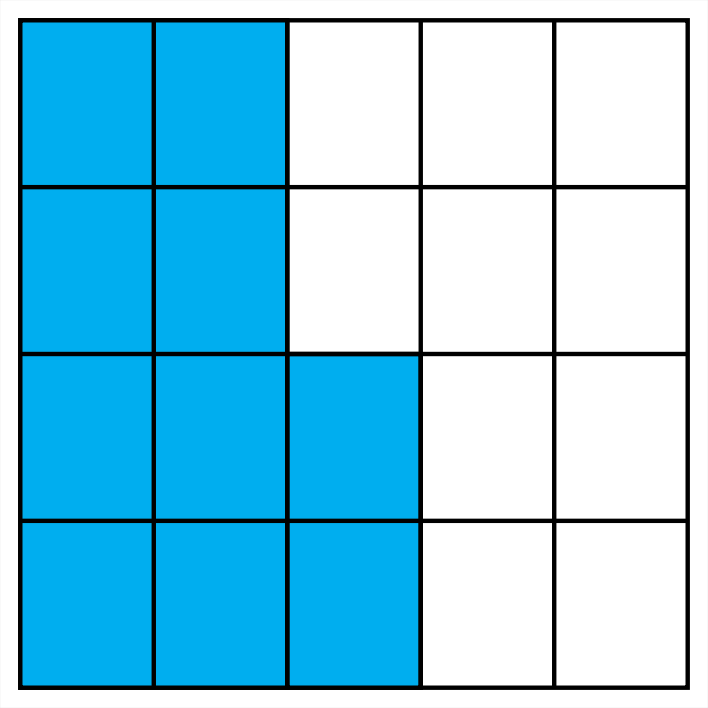
\includegraphics[width=48px]{../images/imagen_frac01.png} \fillin[\fbox{$\dfrac{10}{20}$}][0in]   \\[2em]
				\part 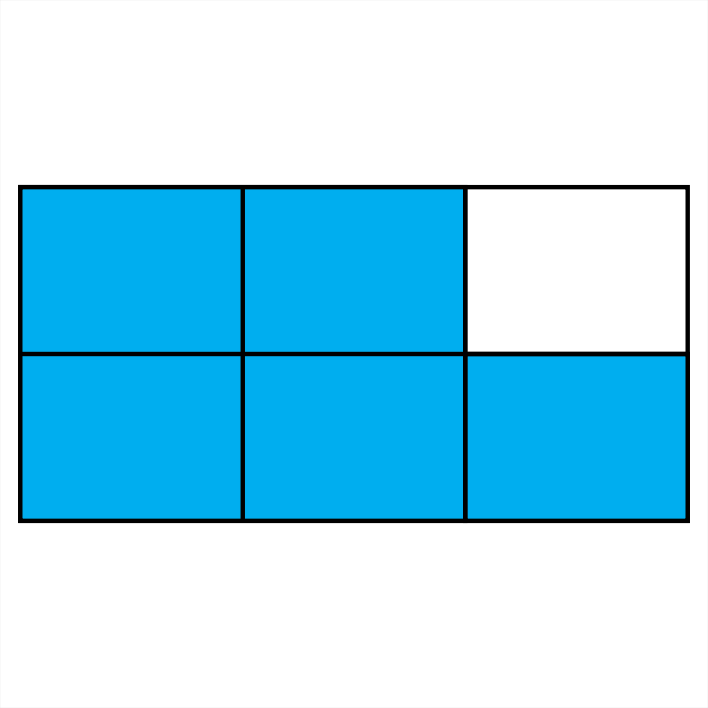
\includegraphics[width=48px]{../images/imagen_frac02.png} \fillin[\fbox{$\dfrac{5}{6}$}][0in]     \\[2em]
				\part 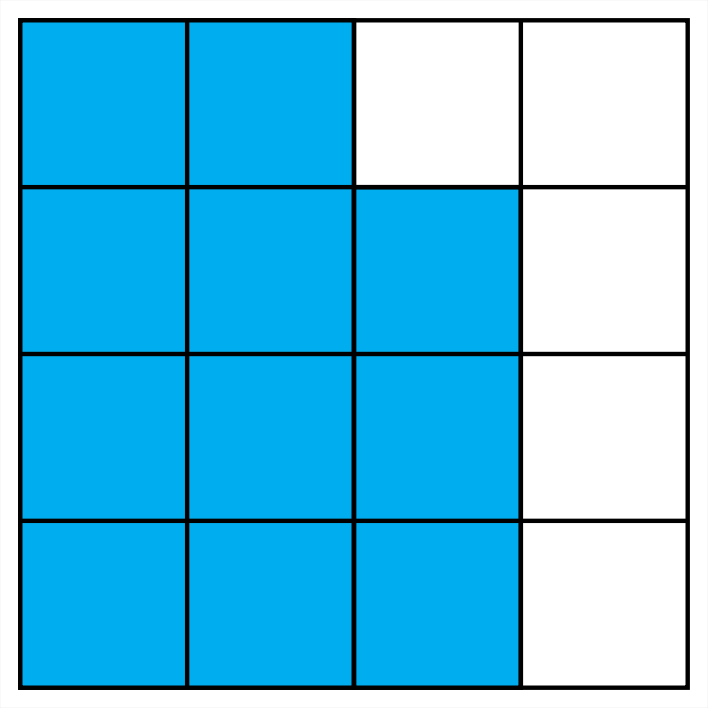
\includegraphics[width=48px]{../images/imagen_frac03.png} \fillin[\fbox{$\dfrac{11}{16}$}][0in]   \\[2em]
				\part 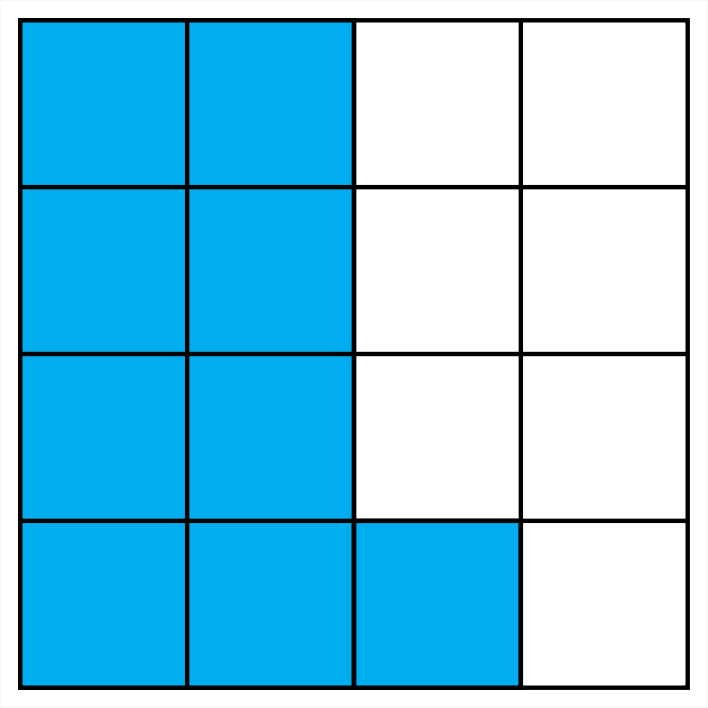
\includegraphics[width=48px]{../images/imagen_frac06.png} \fillin[\fbox{$\dfrac{9}{16}$}][0in]    \\[2em]
				\part 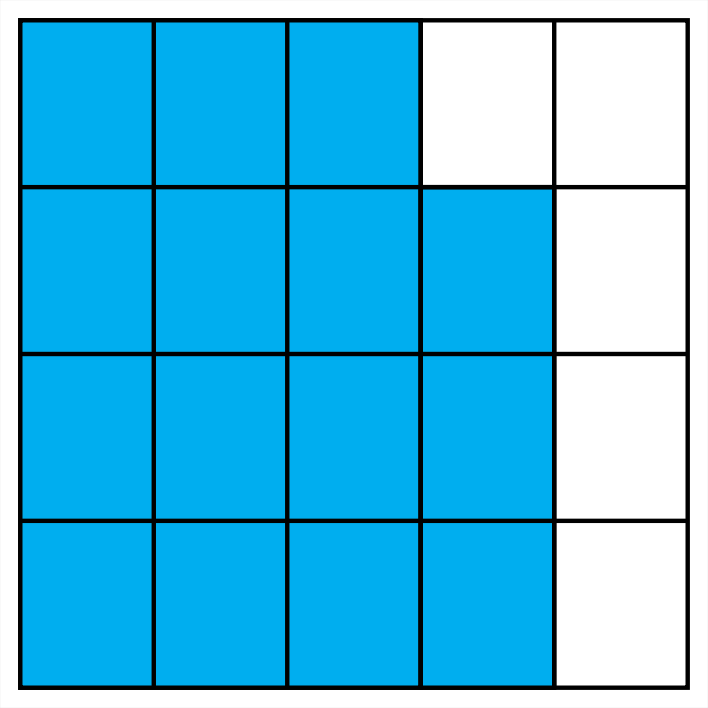
\includegraphics[width=48px]{../images/imagen_frac07.png} \fillin[\fbox{$\dfrac{15}{20}$}][0in]   \\[2em]
				\part 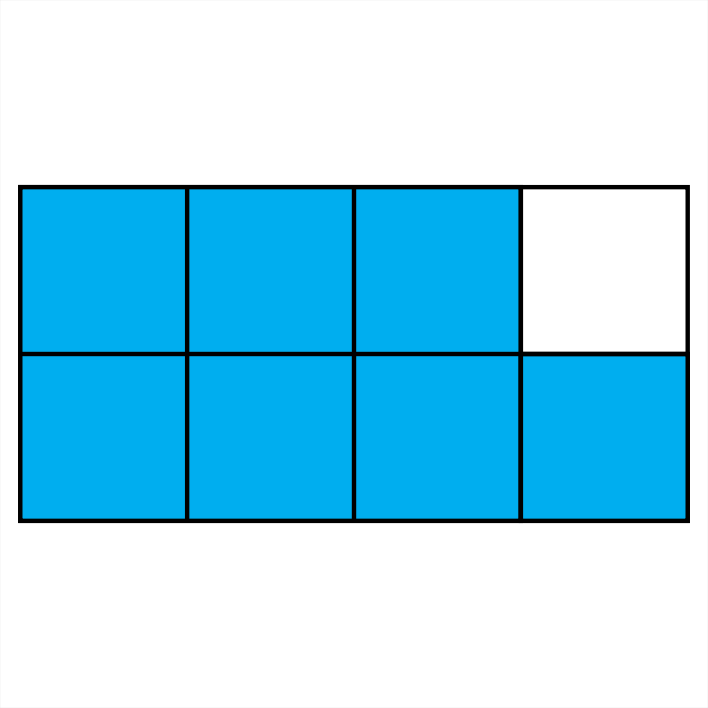
\includegraphics[width=48px]{../images/imagen_frac08.png} \fillin[\fbox{$\dfrac{7}{8}$}][0in]     \\[2em]
				\part 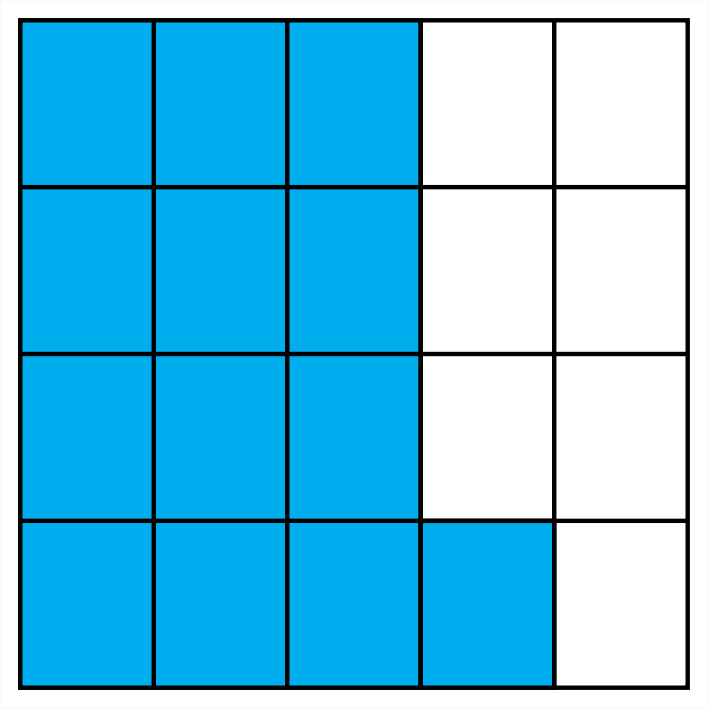
\includegraphics[width=48px]{../images/imagen_frac09.png} \fillin[\fbox{$\dfrac{13}{20}$}][0in]   \\[2em]
				\part 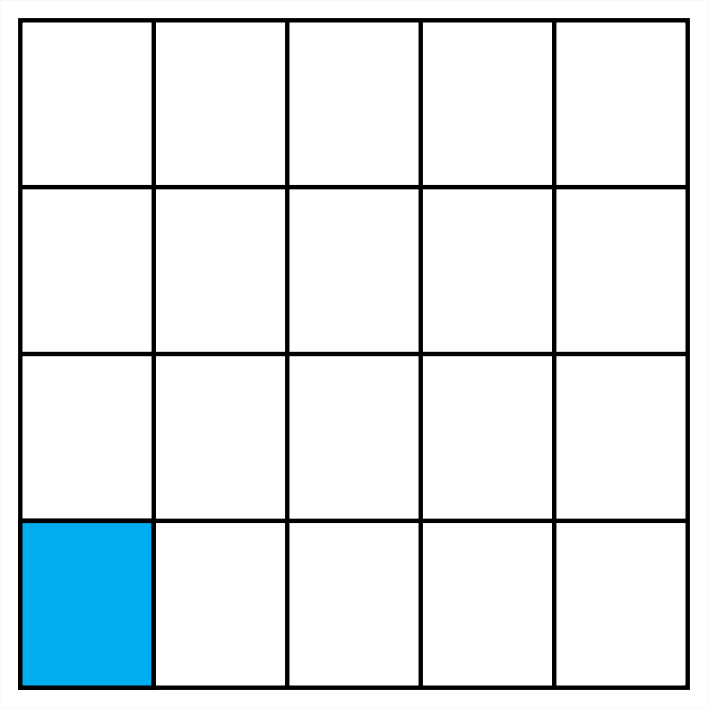
\includegraphics[width=48px]{../images/imagen_frac11.png} \fillin[\fbox{$\dfrac{1}{20}$}][0in]    \\[2em]
			\end{parts}
		\end{multicols}
	}


	% \subsubNombre de fracciones                       }

	\question[4]{Escribe la fracción que corresponda en cada inciso:

		\begin{parts}
			\part ¿Cómo se escribe numéricamente la fracción ocho quintos?    \fillin[$\dfrac{8}{5}$][0in]  \\[1em]
			\part ¿Cómo se escribe numéricamente la fracción seis onceavos?   \fillin[$\dfrac{6}{11}$][0in] \\[1em]
			\part ¿Cómo se escribe numéricamente la fracción dos séptimos?    \fillin[$\dfrac{2}{7}$][0in]  \\[1em]
			\part ¿Cómo se escribe numéricamente la fracción once medios?     \fillin[$\dfrac{11}{2}$][0in] \\[1em]
			% \part ¿Cómo se escribe numéricamente la fracción diez décimos?    \fillin[$\dfrac{10}{10}$][0in]\\[1em]
		\end{parts}
	}

	% \subsubConversión de fracciones mixtas a impropias}

	\question[3]{Convierte la siguientes fracciones mixtas a impropias:

		\begin{multicols}{3}
			\begin{parts}%\large
				\part $4\dfrac{2}{3}= $ \fillin[$\dfrac{14}{3}$][0in ]\\[0.4em]

				\part $2\dfrac{3}{10}= $ \fillin[$\dfrac{23}{10}$][0in ]\\[0.4em]

				\part $5\dfrac{1}{5}= $ \fillin[$\dfrac{26}{5}$][0in] \\[0.4em]
			\end{parts}
		\end{multicols}
	}

	% \subsubConversión de fracciones impropias a mixtas}

	\question[3]{Convierte la siguientes fracciones impropias a mixtas:

		\begin{multicols}{3}
			\begin{parts}%\large
				\part $\dfrac{13}{3}= $ \fillin[$4\dfrac{1}{3}$][0in] \\[0.4em]

				\part $\dfrac{63}{10}= $ \fillin[$6\dfrac{3}{10}$][0in] \\[0.4em]

				\part $\dfrac{51}{5}= $ \fillin[$10\dfrac{1}{5}$][0in] \\[0.4em]
			\end{parts}
		\end{multicols}
	}

	% \subOperaciones con fracciones                 }
	% \subsubSuma de fracciones                         }
	% \subsubResta de fracciones                        }
	% \subsubMultiplicación de fracciones               }
	% \subsubDivisión de fracciones                     }
	% \subsubOperaciones de fracciones mixtas           }

\newpage
	\addcontentsline{toc}{subsection}{Operaciones con fracciones}
	\subsection*{Operaciones con fracciones}

	\question[8]{Realiza las siguientes operaciones.

		\begin{multicols}{2}
			\begin{parts}%\large
				\part $\dfrac{3}{5}+\dfrac{4}{5}=$ \fillin[$\dfrac{7}{5} = 1\dfrac{2}{5}$][0in] \\[2em]
				\part $\dfrac{13}{6}-\dfrac{5}{6}=$ \fillin[$\dfrac{8}{6}=\dfrac{4}{3}$][0in] \\[2em]
				\part $\dfrac{12}{7}-\dfrac{5}{7}=$ \fillin[$\dfrac{7}{7}=1$][0in] \\[2em]
				\part $1\dfrac{1}{8}+1\dfrac{7}{8}=$ \fillin[$2\dfrac{8}{8} = 3$][0in] \\[2em]
				\part $\dfrac{3}{5}\times\dfrac{2}{3}=$ \fillin[$\dfrac{6}{15}$][0in]   \\[2em]
				\part $\dfrac{7}{8}\times\dfrac{3}{4}=$ \fillin[$\dfrac{21}{32}$][0in] \\[2em]
				\part $\dfrac{3}{5} \divisionsymbol\dfrac{2}{3}=$ \fillin[$\dfrac{9}{10}$][0in] \\[2em]
				\part $\dfrac{7}{8} \divisionsymbol\dfrac{3}{4}=$ \fillin[$\dfrac{28}{24}$][0in]	\\[2em]
			\end{parts}
		\end{multicols}
	}
\end{questions}
\end{document}